\documentclass{tufte-handout}

\title{CS224n: Natural Language Processing with Deep Learning\thanks{Course Instructors: Christopher Manning, Richard Socher}}

\author[Francois Chaubard, Rohit Mundra, Richard Socher]{Lecture Notes: Part I\thanks{Authors: Francois Chaubard, Rohit Mundra, Richard Socher}}

\date{Winter 2017} % without \date command, current date is supplied

%\geometry{showframe} % display margins for debugging page layout

\usepackage{graphicx} % allow embedded images
  \setkeys{Gin}{width=\linewidth,totalheight=\textheight,keepaspectratio}
  \graphicspath{{notes1/fig/}} % set of paths to search for images
\usepackage{amsmath}  % extended mathematics
\usepackage{amstext}  % extended text
\usepackage{booktabs} % book-quality tables
\usepackage{units}    % non-stacked fractions and better unit spacing
\usepackage{multicol} % multiple column layout facilities
\usepackage{lipsum}   % filler text
\usepackage{fancyvrb} % extended verbatim environments
\usepackage{placeins}
\usepackage{sty/kbordermatrix}

  \fvset{fontsize=\normalsize}% default font size for fancy-verbatim environments

% Standardize command font styles and environments
\newcommand{\doccmd}[1]{\texttt{\textbackslash#1}}% command name -- adds backslash automatically
\newcommand{\docopt}[1]{\ensuremath{\langle}\textrm{\textit{#1}}\ensuremath{\rangle}}% optional command argument
\newcommand{\docarg}[1]{\textrm{\textit{#1}}}% (required) command argument
\newcommand{\docenv}[1]{\textsf{#1}}% environment name
\newcommand{\docpkg}[1]{\texttt{#1}}% package name
\newcommand{\doccls}[1]{\texttt{#1}}% document class name
\newcommand{\docclsopt}[1]{\texttt{#1}}% document class option name
\newenvironment{docspec}{\begin{quote}\noindent}{\end{quote}}% command specification environment
\newcommand{\argmin}{\operatornamewithlimits{argmin}}
\newcommand{\argmax}{\operatornamewithlimits{argmax}}
\newcommand{\textunderscript}[1]{$_{\text{#1}}$}

\setcounter{secnumdepth}{3}

\begin{document}

\maketitle% this prints the handout title, author, and date

%\printclassoptions


\textbf{Keyphrases: Natural Language Processing. Word Vectors. Singular Value Decomposition. Skip-gram. Continuous Bag of Words (CBOW). Negative Sampling. Hierarchical Softmax. Word2Vec.}

This set of notes begins by introducing the concept of Natural Language Processing (NLP) and the problems NLP faces today. We then move forward to discuss the concept of representing words as numeric vectors. Lastly, we discuss popular approaches to designing word vectors.

% TODO
% should we move SVD methods to the lecture notes 2 (to follow chronological order)??
% should we add a table of content?
% \tableofcontents

\section{Introduction to Natural Language Processing}\label{sec:intro-nlp}

\marginnote{Natural Language Processing tasks come in varying levels of difficulty:
\begin{itemize}
\item [\textbf{Easy}]
\item Spell Checking
\item Keyword Search
\item Finding Synonyms
\item [\textbf{Medium}]
\item Parsing information from websites, documents, etc.
\item [\textbf{Hard}]
\item Machine Translation
\item Semantic Analysis
\item Coreference
\item Question Answering
\end{itemize}
}

We begin with a general discussion of what is NLP. The goal of NLP is to be able to design algorithms to allow computers to "understand" natural language in order to perform some task. Example tasks come in varying level of difficulty:


\begin{itemize}
\item [\textbf{Easy}]
\item Spell Checking
\item Keyword Search
\item Finding Synonyms
\item [\textbf{Medium}]
\item Parsing information from websites, documents, etc.
\item [\textbf{Hard}]
\item Machine Translation (e.g. Translate Chinese text to English)
\item Semantic Analysis (What is the meaning of query statement?)
\item Coreference (e.g. What does "he" or "it" refer to given a document?) 
\item Question Answering (e.g. Answering Jeopardy questions).
\end{itemize}

What's so special about human language? Human language is a system specifically constructed to convey meaning, and is not produced by a physical manifestation of any kind. In that way, it is very different from vision or any other machine learning task. It is a discrete/symbolic/categorical signaling system. Most of the words are just symbols for an extra-linguistic entity. For instance, the word "rocket" refers to the concept of a rocket, and by extension can designates an instance of a rocket. A lot of work in linguistics has been done to conceptualize human language and distinguish the words from their reference, their meaning, etc. ... (Among others, Wittgenstein, Frege, Russel and Mill).
% TODO, include a few references

The first and arguably most important common denominator across all NLP tasks is how we represent words as input to any and all of our models. Much of the earlier NLP work that we will not cover treats words as atomic symbols. To perform well on most NLP tasks we first need to have some notion of similarity and difference between words. With word vectors, we can quite easily encode this ability in the vectors themselves (using distance measures such as Jaccard, Cosine, Euclidean, etc).

\section{Word Vectors}\label{sec:wordvectors}

There are an estimated 13 million tokens for the English language but are they all completely unrelated? Feline to cat, hotel to motel? I think not. Thus, we want to encode word tokens each into some vector that represents a point in some sort of "word" space. This is paramount for a number of reasons but the most intuitive reason is that perhaps there actually exists some $N$-dimensional space (such that $N\ll13$ million) that is sufficient to encode all semantics of our language. Each dimension would encode some meaning that we transfer using speech. For instance, semantic dimensions might indicate tense (past vs. present vs. future), count (singular vs. plural), and gender (masculine vs. feminine). 

\marginnote{\textbf{One-hot} vector: Represent every word as an $\mathbb{R}^{|V|\times1}$ vector with all $0$s and one $1$ at the index of that word in the sorted english language.}

So let's dive into our first word vector and arguably the most simple, the \textbf{one-hot vector}: Represent every word as an $\mathbb{R}^{|V|\times1}$ vector with all $0$s and one $1$ at the index of that word in the sorted english language. In this notation, $|V|$ is the size of our vocabulary. Word vectors in this type of encoding would appear as the following:

$w^{aardvark} = \left[ \begin{array}{c} 1 \\ 0 \\ 0 \\ \vdots \\ 0 \end{array} \right]$, $w^{a} = \left[ \begin{array}{c} 0 \\ 1 \\ 0 \\ \vdots \\ 0 \end{array} \right] $, $w^{at} = \left[ \begin{array}{c} 0 \\ 0 \\ 1 \\ \vdots \\ 0 \end{array} \right] $, $\cdots$ $w^{zebra} = \left[ \begin{array}{c} 0 \\ 0 \\ 0 \\ \vdots \\ 1 \end{array} \right] $

\marginnote{\textbf{Fun fact:} The term "one-hot" comes from digital circuit design, meaning "a group of bits among which the legal combinations of values are only those with a single high (1) bit and all the others low (0)".}

We represent each word as a completely independent entity. As we previously discussed, this word representation does not give us directly any notion of similarity. For instance,

$$(w^{hotel})^Tw^{motel} = (w^{hotel})^Tw^{cat} = 0$$

So maybe we can try to reduce the size of this space from $\mathbb{R}^|V|$ to something smaller and thus find a subspace that encodes the relationships between words.

\section{SVD Based Methods}\label{sec:svdmethods}

For this class of methods to find word embeddings (otherwise known as word vectors), we first loop over a massive dataset and accumulate word co-occurrence counts in some form of a matrix $X$, and then perform Singular Value Decomposition on $X$ to get a $USV^T$ decomposition. We then use the rows of $U$ as the word embeddings for all words in our dictionary. Let us discuss a few choices of $X$.

\subsection{Word-Document Matrix}
As our first attempt, we make the bold conjecture that words that are related will often appear in the same documents. For instance, "banks", "bonds", "stocks", "money", etc. are probably likely to appear together. But "banks", "octopus", "banana", and "hockey" would probably not consistently appear together. We use this fact to build a word-document matrix, $X$ in the following manner: Loop over billions of documents and for each time word $i$ appears in document $j$, we add one to entry $X_{ij}$. This is obviously a very large matrix ($\mathbb{R}^{|V|\times M}$) and it scales with the number of documents ($M$). So perhaps we can try something better.

\subsection{Window based Co-occurrence Matrix}
The same kind of logic applies here however, the matrix $X$ stores co-occurrences of words thereby becoming an affinity matrix. In this method we count the number of times each word appears inside a window of a particular size around the word of interest. We calculate this count for all the words in corpus. We display an example below. Let our corpus contain just three sentences and the window size be 1:

\marginnote{\textbf{Using Word-Word Co-occurrence Matrix:}\\
\begin{itemize}
\item Generate $|V|\times|V|$ co-occurrence matrix, $X$.
\item Apply SVD on $X$ to get $X = USV^T$.
\item Select the first $k$ columns of $U$ to get a $k$-dimensional word vectors.
\item $\frac{\sum_{i = 1}^{k}\sigma_i}{\sum_{i = 1}^{|V|}\sigma_i}$ indicates the amount of variance captured by the first $k$ dimensions.
\end{itemize}
}

\begin{enumerate}
\item I enjoy flying.
\item I like NLP.
\item I like deep learning.
\end{enumerate}

The resulting counts matrix will then be:
$$X=\kbordermatrix{
        & I & like & enjoy & deep & learning & NLP & flying & . \\
     I & 0 & 2 & 1 & 0 & 0 & 0 & 0 & 0\\
    like & 2 & 0 & 0 & 1 & 0 & 1 & 0 & 0\\
    enjoy & 1 & 0 & 0 & 0 & 0 & 0 & 1 & 0 \\
    deep & 0 & 1 & 0 & 0 & 1 & 0 & 0 & 0 \\
    learning & 0 & 0 & 0 & 1 & 0 & 0 & 0 & 1\\
    NLP & 0 & 1 & 0 & 0 & 0 & 0 & 0 & 1\\
    flying & 0 & 0 & 1 & 0 & 0 & 0 & 0 & 1\\
    . & 0 & 0 & 0 & 0 & 1 & 1 & 1 & 0
  }$$

We now perform SVD on $X$, observe the singular values (the diagonal entries in the resulting $S$ matrix), and cut them off at some index $k$ based on the desired percentage variance captured:
$$\frac{\sum_{i = 1}^{k}\sigma_i}{\sum_{i = 1}^{|V|}\sigma_i}$$
We then take the submatrix of $U_{1:|V|,1:k}$ to be our word embedding matrix. This would thus give us a $k$-dimensional representation of every word in the vocabulary.
$$$$
\textbf{Applying SVD to $X$}:
$$\kbordermatrix{
        & & |V| & \\
       & \\
       |V| & & X \\
       & \\
       } =  \kbordermatrix{
        & & |V| & \\
       & | & |\\
       |V| & u_1 & u_2 & \cdots\\
       & | & |\\
       }  \kbordermatrix{
        & & |V| & \\
       & \sigma_1 & 0 & \cdots\\
       |V| & 0 & \sigma_2 & \cdots\\
       & \vdots & \vdots & \ddots\\
       }
       \kbordermatrix{
        & & |V| & \\
       & - & v_1 & -\\
       |V| & - & v_2 & -\\
       & & \vdots\\
       }
$$
\textbf{Reducing dimensionality by selecting first $k$ singular vectors}:
$$\kbordermatrix{
        & & |V| & \\
       & \\
       |V| & & \hat{X} \\
       & \\
       } =  \kbordermatrix{
        & & k & \\
       & | & |\\
       |V| & u_1 & u_2 & \cdots\\
       & | & |\\
       }  \kbordermatrix{
        & & k & \\
       & \sigma_1 & 0 & \cdots\\
       k & 0 & \sigma_2 & \cdots\\
       & \vdots & \vdots & \ddots\\
       }
       \kbordermatrix{
        & & |V| & \\
       & - & v_1 & -\\
       k & - & v_2 & -\\
       & & \vdots\\
       }
$$

Both of these methods give us word vectors that are more than sufficient to encode semantic and syntactic (part of speech) information but are associated with many other problems:
\begin{itemize}
\item The dimensions of the matrix change very often (new words are added very frequently and corpus changes in size).
\item The matrix is extremely sparse since most words do not co-occur.
\item The matrix is very high dimensional in general ($\approx 10^6 \times 10^6$)
\item Quadratic cost to train (i.e. to perform SVD)
\item Requires the incorporation of some hacks on $X$ to account for the drastic imbalance in word frequency
\end{itemize}
Some solutions to exist to resolve some of the issues discussed above:
\begin{itemize}
\item Ignore function words such as "the", "he", "has", etc.
\item Apply a ramp window -- i.e. weight the co-occurrence count based on distance between the words in the document. 
\item Use Pearson correlation and set negative counts to 0 instead of using just raw count.
\end{itemize}

As we see in the next section, iteration based methods solve many of these issues in a far more elegant manner.

\section{Iteration Based Methods}\label{sec:itermethods}

Let us step back and try a new approach. Instead of computing and storing global information about some huge dataset (which might be billions of sentences), we can try to create a model that will be able to learn one iteration at a time and eventually be able to encode the probability of a word given its context. 

\marginnote{\textbf{Context of a word:}\\
The context of a word is the set of $C$ surrounding words. For instance, the $C = 2$ context of the word "fox" in the sentence "The quick brown fox jumped over the lazy dog" is \{"quick", "brown", "jumped", "over"\}.}

We can set up this probabilistic model of known and unknown parameters and take one training example at a time in order to learn just a little bit of information for the unknown parameters based on the input, the output of the model, and the desired output of the model.

At every iteration we run our model, evaluate the errors, and follow an update rule that has some notion of penalizing the model parameters that caused the error. This idea is a very old one dating back to 1986. We call this method "backpropagating" the errors (see \textsc{Learning representations by back-propagating errors. David E. Rumelhart, Geoffrey E. Hinton, and Ronald J. Williams (1988).})

\subsection{Language Models (Unigrams, Bigrams, etc.)}
First, we need to create such a model that will assign a probability to a sequence of tokens. Let us start with an example:

\begin{center}
\textit{"The cat jumped over the puddle."}
\end{center}

A good language model will give this sentence a high probability because this is a completely valid sentence, syntactically and semantically. Similarly, the sentence "stock boil fish is toy" should have a very low probability because it makes no sense. Mathematically, we can call this probability on any given sequence of $n$ words:
$$P(w_{1}, w_{2}, \cdots, w_{n})$$
We can take the unary language model approach and break apart this probability by assuming the word occurrences are completely independent:
$$P(w_{1}, w_{2}, \cdots, w_{n}) = \prod_{i=1}^n P(w_{i})$$

\marginnote{\textbf{Unigram model:}
$$P(w_{1}, w_{2}, \cdots, w_{n}) = \prod_{i=1}^n P(w_{i})$$}

However, we know this is a bit ludicrous because we know the next word is highly contingent upon the previous sequence of words. And the silly sentence example might actually score highly. So perhaps we let the probability of the sequence depend on the pairwise probability of a word in the sequence and the word next to it. We call this the bigram model and represent it as:

$$P(w_{1}, w_{2}, \cdots, w_{n}) = \prod_{i=2}^n P(w_{i} | w_{i-1})$$

\marginnote{\textbf{Bigram model:}
$$P(w_{1}, w_{2}, \cdots, w_{n}) = \prod_{i=2}^n P(w_{i} | w_{i-1})$$}

Again this is certainly a bit naive since we are only concerning ourselves with pairs of neighboring words rather than evaluating a whole sentence, but as we will see, this representation gets us pretty far along. Note in the Word-Word Matrix with a context of size 1, we basically can learn these pairwise probabilities. But again, this would require computing and storing global information about a massive dataset.

Now that we understand how we can think about a sequence of tokens having a probability, let us observe some example models that could learn these probabilities.

\subsection{Continuous Bag of Words Model (CBOW)}

One approach is to treat \{"The", "cat", 'over", "the', "puddle"\} as a context and from these words, be able to predict or generate the center word "jumped". This type of model we call a Continuous Bag of Words (CBOW) Model.

\marginnote{\textbf{CBOW Model:}\\Predicting a center word form the surrounding context}

Let's discuss the CBOW Model above in greater detail. First, we set up our known parameters. Let the known parameters in our model be the sentence represented by one-hot word vectors. The input one hot vectors or context we will represent with an $x^{(c)}$. And the output as $y^{(c)}$ and in the CBOW model, since we only have one output, so we just call this $y$ which is the one hot vector of the known center word. Now let's define our unknowns in our model. 

\marginnote{\textbf{Notation for CBOW Model:}\\
\begin{itemize}
\item $w_{i}$: Word $i$ from vocabulary $V$
\item $\mathcal{V} \in \mathbb{R}^{n\times|V|}$: Input word matrix
\item $v_{i}$: $i$-th column of $\mathcal{V}$, the input vector representation of word $w_{i}$
\item $\mathcal{U} \in \mathbb{R}^{n\times|V|}$: Output word matrix
\item $u_{i}$: $i$-th row of $\mathcal{U}$, the output vector representation of word $w_{i}$

\end{itemize}
}

We create two matrices, $\mathcal{V} \in \mathbb{R}^{n\times|V|}$ and $\mathcal{U} \in \mathbb{R}^{|V|\times n}$. Where $n$ is an arbitrary size which defines the size of our embedding space. $\mathcal{V}$ is the input word matrix such that the $i$-th column of $\mathcal{V}$ is the $n$-dimensional embedded vector for word $w_{i}$ when it is an input to this model. We denote this $n\times1$ vector as $v_{i}$. Similarly, $\mathcal{U}$ is the output word matrix. The $j$-th row of $\mathcal{U}$ is an $n$-dimensional embedded vector for word $w_{j}$ when it is an output of the model. We denote this row of $\mathcal{U}$ as $u_{j}$. Note that we do in fact learn two vectors for every word $w_{i}$ (i.e. input word vector $v_{i}$ and output word vector $u_{i}$).
$$ $$
We breakdown the way this model works in these steps:
\begin{enumerate}
\item We generate our one hot word vectors ($x^{(c-m)}, \hdots, x^{(c-1)}, x^{(c+1)},\hdots, x^{(c+m)}$) for the input context of size $m$.
\item We get our embedded word vectors for the context ($v_{c-m}=\mathcal{V}x^{(c-m)}$, $v_{c-m+1}=\mathcal{V}x^{(c-m+1)}$, $\hdots$, $v_{c+m}=\mathcal{V}x^{(c+m)}$) 
\item Average these vectors to get $\hat{v} = \frac{v_{c-m}+v_{c-m+1}+... + v_{c+m}}{2m}$
\item Generate a score vector $z=\mathcal{U}\hat{v}$
\item Turn the scores into probabilities $\hat{y}=\operatorname{softmax}(z)$
\item We desire our probabilities generated, $\hat{y}$, to match the true probabilities, $y$, which also happens to be the one hot vector of the actual word.
\end{enumerate}

\begin{marginfigure}%
  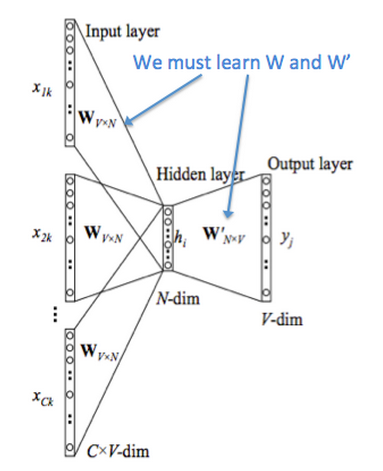
\includegraphics[width=\linewidth]{CBOW}
  \caption{This image demonstrates how CBOW works and how we must learn the transfer matrices}
  \label{fig:CBOW}
\end{marginfigure}

So now that we have an understanding of how our model would work if we had a $\mathcal{V}$ and $\mathcal{U}$, how would we learn these two matrices? Well, we need to create an objective function. Very often when we are trying to learn a probability from some true probability, we look to information theory to give us a measure of the distance between two distributions. Here, we use a popular choice of distance/loss measure, cross entropy $H(\hat{y},y)$. 

The intuition for the use of cross-entropy in the discrete case can be derived from the formulation of the loss function:
$$H(\hat{y},y) = -\sum_{j = 1}^{|V|} y_j \log(\hat{y}_j)$$
Let us concern ourselves with the case at hand, which is that $y$ is a one-hot vector. Thus we know that the above loss simplifies to simply:
$$H(\hat{y},y) = -y_i \log(\hat{y}_i)$$

In this formulation, $c$ is the index where the correct word's one hot vector is $1$. We can now consider the case where our prediction was perfect and thus $\hat{y}_c = 1$. We can then calculate $H(\hat{y},y) = -1\log(1) = 0$. Thus, for a perfect prediction, we face no penalty or loss. Now let us consider the opposite case where our prediction was very bad and thus $\hat{y}_c = 0.01$. As before, we can calculate our loss to be $H(\hat{y},y) = -1\log(0.01) \approx 4.605$. We can thus see that for probability distributions, cross entropy provides us with a good measure of distance. We thus formulate our optimization objective as:
\begin{align*}
\operatorname{minimize} J &= -\log P(w_{c}|w_{c-m}, \hdots, w_{c-1}, w_{c+1}, \hdots, w_{c+m})\\
&= -\log P(u_{c}|\hat{v})\\
&= -\log \frac{\exp(u_{c}^{T}\hat{v})}{\sum_{j=1}^{|V|}\exp(u_{j}^{T}\hat{v})}\\
&= -u_{c}^{T}\hat{v}+\log \sum_{j=1}^{|V|}\exp(u_{j}^{T}\hat{v})\\
\end{align*}
We use gradient descent to update all relevant word vectors $u_{c}$ and $v_{j}$.\\

%[To be added after Assignment $1$ is graded]

\subsection{Skip-Gram Model}

\marginnote{\textbf{Skip-Gram Model:}\\Predicting surrounding context words given a center word}


Another approach is to create a model such that given the center word "jumped", the model will be able to predict or generate the surrounding words "The", "cat", "over", "the", "puddle". Here we call the word "jumped" the context. We call this type of model a Skip-Gram model.

\marginnote{\textbf{Notation for Skip-Gram Model:}\\
\begin{itemize}
\item $w_i$: Word $i$ from vocabulary $V$
\item $\mathcal{V} \in \mathbb{R}^{n\times|V|}$: Input word matrix
\item $v_i$: $i$-th column of $\mathcal{V}$, the input vector representation of word $w_i$
\item $\mathcal{U} \in \mathbb{R}^{n\times|V|}$: Output word matrix
\item $u_i$: $i$-th row of $\mathcal{U}$, the output vector representation of word $w_i$
\end{itemize}
}

Let's discuss the Skip-Gram model above. The setup is largely the same but we essentially swap our $x$ and $y$ i.e. $x$ in the CBOW are now $y$ and vice-versa. The input one hot vector (center word) we will represent with an $x$ (since there is only one). And the output vectors as $y^{(j)}$. We define $\mathcal{V}$ and $\mathcal{U}$ the same as in CBOW.
\vspace{-.5cm}
$$ $$
We breakdown the way this model works in these 6 steps:
\begin{enumerate}
\item We generate our one hot input vector $x$
\item We get our embedded word vectors for the context $v_{c} =\mathcal{V}x$
\item Since there is no averaging, just set $\hat{v} = v_{c}$
?\item Generate $2m$ score vectors, $u_{c-m}, \hdots, u_{c-1}, u_{c+1}, \hdots, u_{c+m}$ using $u=\mathcal{U}v_{c}$
\item Turn each of the scores into probabilities, $y = \operatorname{softmax}(u)$
\item We desire our probability vector generated to match the true probabilities which is
$y^{(c-m)}, \hdots, y^{(c-1)}, y^{(c+1)}, \hdots, y^{(c+m)}$, the one hot vectors of the actual output.
\end{enumerate}

As in CBOW, we need to generate an objective function for us to evaluate the model. A key difference here is that we invoke a Naive Bayes assumption to break out the probabilities. If you have not seen this before, then simply put, it is a strong (naive) conditional independence assumption. In other words, given the center word, all output words are completely independent.

\begin{marginfigure}%
  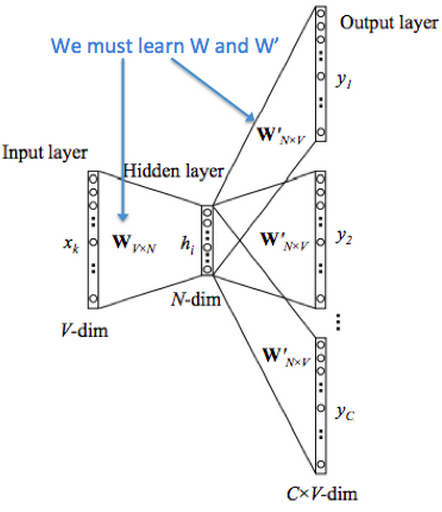
\includegraphics[width=\linewidth]{Skip-Gram}
  \caption{This image demonstrates how Skip-Gram works and how we must learn the transfer matrices}
  \label{fig:Skipgram}
\end{marginfigure}

\begin{align*}
\operatorname{minimize} J &= -\log P(w_{c-m}, \hdots, w_{c-1}, w_{c+1}, \hdots, w_{c+m}|w_{c})\\
&= -\log \prod_{j=0, j\neq m}^{2m} P(w_{c-m+j}|w_{c})\\
&= -\log \prod_{j=0, j\neq m}^{2m} P(u_{c-m+j}|v_{c})\\
&= -\log \prod_{j=0, j\neq m}^{2m} \frac{\exp(u_{c-m+j}^{T}v_{c})}{\sum_{k=1}^{|V|}\exp(u_{k}^{T}v_{c})}\\
&= -\sum_{j=0, j\neq m}^{2m} u_{c-m+j}^{T}v_{c} + 2m\log \sum_{k=1}^{|V|}\exp(u_{k}^{T}v_{c})\\
\end{align*}
With this objective function, we can compute the gradients with respect to the unknown
parameters and at each iteration update them via Stochastic Gradient Descent.

%[To be added after Assignment $1$ is graded]

\subsection{Negative Sampling}

Lets take a second to look at the objective function. Note that the summation over $|V|$ is computationally huge! Any update we do or evaluation of the objective function would take $O(|V|)$ time which if we recall is in the millions. A simple idea is we could instead just approximate it.

For every training step, instead of looping over the entire vocabulary, we can just sample several negative examples! We "sample" from a noise distribution ($P_n(w)$) whose probabilities match the ordering of the frequency of the vocabulary. To augment our formulation of the problem to incorporate Negative Sampling, all we need to do is update the:
\begin{itemize}
\item objective function
\item gradients
\item update rules
\end{itemize}

\textsc{Mikolov et al.} present \textbf{Negative Sampling} in \textsc{Distributed Representations of Words and Phrases and their Compositionality}. While negative sampling is based on the Skip-Gram model, it is in fact optimizing a different objective. Consider a pair $(w, c)$ of word and context. Did this pair come from the training data? Let's denote by $P(D = 1|w, c)$ the probability that (w, c) came from the corpus data. Correspondingly, $P(D = 0|w, c)$ will be the probability that $(w, c)$ did not come from the corpus data. First, let's model $P(D = 1|w, c)$ with the sigmoid function:
$$ P(D = 1|w, c, \theta) = \frac{1}{1+ e^{(-v_c^Tv_w)}}$$
Now, we build a new objective function that tries to maximize the probability of a word and context being in the corpus data if it indeed is, and maximize the probability of a word and context not being in the corpus data if it indeed is not. We take a simple maximum likelihood approach of these two probabilities. (Here we take $\theta$ to be the parameters of the model, and in our case it is $\mathcal{V}$ and $\mathcal{U}$.)
\begin{align*}
\theta &= \argmax_{\theta} \prod_{(w,c) \in D} P(D = 1|w, c, \theta) \prod_{(w,c) \in \tilde{D}} P(D = 0|w, c, \theta) \\
&= \argmax_{\theta} \prod_{(w,c) \in D} P(D = 1|w, c, \theta) \prod_{(w,c) \in \tilde{D}} (1 - P(D = 1|w, c, \theta))\\
&= \argmax_{\theta} \sum_{(w,c) \in D} \log P(D = 1|w, c, \theta) + \sum_{(w,c) \in \tilde{D}} \log(1 - P(D = 1|w, c, \theta))\\
&= \argmax_{\theta} \sum_{(w,c) \in D} \log \frac{1}{1 + \exp(-u_w^Tv_c)} + \sum_{(w,c) \in \tilde{D}} \log(1 - \frac{1}{1 + \exp(-u_w^Tv_c)} )\\
&= \argmax_{\theta} \sum_{(w,c) \in D} \log \frac{1}{1 + \exp(-u_w^Tv_c)} + \sum_{(w,c) \in \tilde{D}} \log(\frac{1}{1 + \exp(u_w^Tv_c)} )\\
\end{align*}
Note that $\tilde{D}$ is a "false" or "negative" corpus. Where we would have sentences like "stock boil fish is toy". Unnatural sentences that should get a low probability of ever occurring. We can generate $\tilde{D}$ on the fly by randomly sampling this negative from the word bank. Our new objective function would then be:
$$ \log \sigma (u_{c-m+j}^{T}\cdot v_{c})+ \sum_{k = 1}^K \log \sigma (- \tilde{u}_{k}^{T}\cdot v_{c}) $$
In the above formulation, $\{\tilde{u}_{k} | k = 1\hdots K\}$ are sampled from $P_n(w)$. Let's discuss what $P_n(w)$ should be. While there is much discussion of what makes the best approximation, what seems to work best is the Unigram Model raised to the power of 3/4. Why 3/4? Here's an example that might help gain some intuition:\\
\begin{center}
is: $0.9^{3/4} = 0.92$\\
Constitution: $0.09^{3/4} = 0.16$\\
bombastic: $0.01^{3/4} = 0.032$\\
\end{center}

"Bombastic" is now 3x more likely to be sampled while "is" only went up marginally.

\subsection{Hierarchical Softmax}
% TODO


%[Gradients and update rules to be added after Assignment $1$ is graded]
\end{document}
